
\section{Tandem queues}
\label{sec:tandem-queues}

No notes; only exercises.

\begin{question}
  Consider two stations in tandem, as depicted in
  Figure~\ref{fig:tandem}. The service process at both stations is
  subject to variability. Suppose you have some money to spend on
  reducing the variability of either of the two machines.  Which one
  is the better one to spend it on?  You should realize the relevancy
  of modeling for this problem. Due to the lack of money you can only
  realize one of the alternatives; hence there is no way of finding
  out what would have happened if you would have made the other
  choice.

\begin{figure}[htbp]
  \begin{center}
    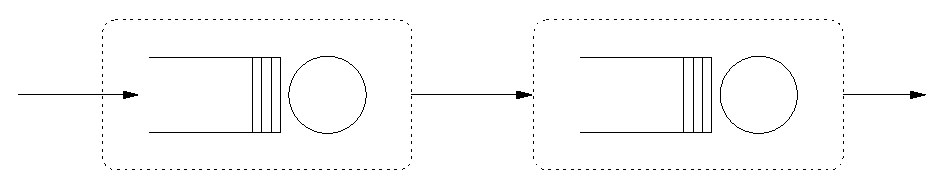
\includegraphics[scale=0.7]{tandem}
    \caption{Jobs arrive at the first station and, after service, move on to the second station.}
    \label{fig:tandem}
  \end{center}
\end{figure}


\begin{solution}
The answer to this problem is of course not clear cut. A well balanced
answer requires some extra information, such as which of the two
stations has the larger variability. However, we can provide some
general insights into this problem.

We first compute the expected waiting time in the queues at both
stations for a  reference situation. Then we derive similar
expressions for the waiting times in case we spend all money on the
second or first station. 

\emph{The reference situation} As a reference scenario, suppose that
the arrival process has a Poisson distribution with rate $\lambda$,
and that the service distributions at the first and second server,
respectively, are exponential with rate $\mu_1$ and $\mu_2$,
respectively. This is, from an analytic point of view, about the
simplest situation we can consider.  We now focus on the waiting times
for each station separately.

The first queue is the familiar $M/M/1$ queue.  (Why?) For the sequel
it is important to observe that the departure process of the first
station, i.e., the distribution of times between jobs leaving the
first station, is the same as the arrival process. Consequently, the
inter-departure times are also exponentially distributed with parameter
$\lambda$. (However, the service times are exponentially distributed
with parameter $\mu_1$. ) This claim can be proved, but is not
immediate. 

What can we say about the second station?  Clearly, the jobs departing
at the first stations are the arrivals at the second station. Hence,
this departure process being exponential with rate $\lambda$, the
inter-arrival times at the second station are also exponential with
rate $\lambda$. Consequently, the second queue is also an $M/M/1$
queue.  

It is well known that, for this case, the total waiting time in the
system, i.e., the time spent in both queues, is the sum of the waiting
times at the first and second station. As each is an $M/M/1$ queue,
the total waiting time has the form:
\begin{equation}
  \begin{split}
E(W)  &= E(W_1) + E(W_2) \\
&= \frac{\rho_1}{1-\rho_1} \frac1{\mu_1} + \frac{\rho_2}{1-\rho_2} \frac1{\mu_2},
  \end{split}
\end{equation}
where $\rho_i = \lambda/\mu_i$ and $E(S_i) = 1/\mu_i$, for $i=1,2$. 


\emph{Case1: Spend all the money on the second server} Now we might
spend the money on the second machine. How would this influence the
total waiting time $E(W)$?

As we reduce the variability of the second server, the service process
is no longer exponential. However, the arrival process at the second
station is still Poisson. As a consequence, the queueing discipline
changes to the $M/G/1$ queue. The expected waiting time for this case
has the form:
\begin{equation}\label{eq:200}
E(W_2) = \frac{1+C_{s,2}^2}2\frac{\rho_2}{1-\rho_2} \frac1{\mu_2},
\end{equation}
where $C_{s,2}$ is the coefficient of variation of the service process
of the second server.  

Suppose the money we have suffices to entirely remove the variability
of the second server.  (This is of course also the best we can
possibly achieve.) This yields that the coefficient of variation
$C_{v,2} = 0$. As an aside, observe that as all variability has been
removed, the service process is entirely deterministic: each service
takes exactly the same amount of time. As a result, we arrive at the
$M/D/1$ queue to model the queueing process at the second station.

The expected waiting time for the $M/D/1$ queue follows immediately
from~(\ref{eq:200}) by setting $C_{v,2} =0$:
\begin{equation}\label{eq:300}
E(W_2) = \frac{1}2\frac{\rho_2}{1-\rho_2} \frac1{\mu_2}.
\end{equation}
Clearly, this is half the waiting time of the  $M/M/1$ queue. 

Since we do not change the first station in any way, this is still an
$M/M/1$ queue. Thus, the total waiting time for this scenario becomes:
\begin{equation*}
  E(W)= \frac{\rho_1}{1-\rho_1} \frac1{\mu_1} +
  \frac12\frac{\rho_2}{1-\rho_2} \frac1{\mu_2}. 
\end{equation*}


\emph{Case 2: Spend the money on the first server} Analogous to the
previous situation, suppose we can set the coefficient of variation
$C_{1,v}$ of the first server to zero. Thus, this becomes an $M/D/1$
queue, so that, similar to~(\ref{eq:300}):
\begin{equation*}
E(W_1) = \frac{1}2\frac{\rho_1}{1-\rho_1} \frac1{\mu_1}.
\end{equation*}

Contrary to the $M/M/1$ queue, the inter-departures of the $M/D/1$
queue are not exponentially distributed. Rather, as long as the first
server is busy, they are deterministic, i.e., equally separated in
time.  Only when the first server is idle---these idle times still
have exponential distribution---there are no regular departures.  Thus
the departure process is not deterministic. However, for the sake of
simplicity, we assume in the sequel that the departure process
\emph{is} deterministic.

As we previously remarked, the departure process of the first station
forms the arrival process at the second station.  Since the departures
are assumed to be deterministic, the arrivals at the second station
are also deterministic.  The service times, however, are still
exponential.  (Recall we do not spend money on the second server to
reduce its variability). Thus, the second station can be modeled as
the $D/M/1$ queue. For this queue we need to derive an expression for
the waiting time. The simplest approximation is follows from an
expression for the waiting time of the $G/G/1$ queue.

It is well known that the expected waiting time for the the $G/G/1$
queue has the approximate form:
\begin{equation}\label{eq:500}
E(W_2) = \frac{C_{a,2}^2+C_{s,2}^2}2\frac{\rho_2}{1-\rho_2} \frac1{\mu_2},
\end{equation}
Clearly, for our case, the coefficient of  variation $C_{a,s}$ of the
arrival process becomes, approximately, $0$, while $C_{s,2} = 1$,
since the service process is still exponential. Hence,
\begin{equation}\label{eq:400}
E(W_2) = \frac12\frac{\rho_2}{1-\rho_2} \frac1{\mu_2}.
\end{equation}

Combining~(\ref{eq:500}) and~(\ref{eq:400}), the total waiting time
becomes:
\begin{equation*}
  E(W)= \frac12\frac{\rho_1}{1-\rho_1} \frac1{\mu_1} +
  \frac12\frac{\rho_2}{1-\rho_2} \frac1{\mu_2}, 
\end{equation*}
which is half the waiting time of the reference scenario, and still
less than the first scenario.

\emph{Conclusion} As a general guide line, it seems best to reduce the
variability at the first station. The main point to remember is that
reducing the variability of the service process at the first station
also reduces the variability of the arrival processes at the second
station. Thus, we gain at two locations of the chain of stations,
rather than at one.

Interestingly, the departure process of the $D/M/1$ queue is not
Poisson; the coefficient of variation is less than $1$. Hence, if
there were a third station, also its input process would behave better
than Poisson. Consequently, reducing variability upstream reduces (in
general) the variability of the arrival processes at all stations
downstream, reducing the waiting time all along the chain. 
\end{solution}
\end{question}


\begin{question}
  (Hall 5.22). At a large hotel, taxi cabs arrive at a rate of 15 per
  hour, and parties of riders arrive at the rate of 12 per
  hour. Whenever taxicabs are waiting, riders are served immediately
  upon arrival. Whenever riders are waiting, taxicabs are loaded
  immediately upon arrival. A maximum of three cabs can wait at a time (other cabs must go elsewhere).
  \begin{enumerate}
  \item Let $p_{ij}$ be the steady-state probability of there being $i$ parties of riders and $j$ taxicabs waiting at the hotel. Write the state transition equation for the system. 
  \item Calculate the expected number of cabs waiting and the expected number of parties waiting.
  \item Calculate the expected waiting time for cabs and the expected waiting for parties. (For cabs, compute the average among those that do not go elsewhere.)
  \item In words, what would be the impact of allowing four cabs to wait at a time?
  \end{enumerate}
  
\hint{ Try to adapt the ideas behind Figure 2.2 of Zijm to this case.}

    \begin{solution}
      \begin{enumerate}
      \item 
This is really a neat problem. Please spend serious time on it to
solve before looking at the answer. It requires some ingenuity on your part. 

Let $p_{ij}$ be the fraction of time that the system contains
$j$ taxi cabs and $i$ riders. I assume that all members of
a party of riders can be served by a single cab (that is, the parties
do not excees the capacity of a cab and all members of a party have
the same destination). For clarity, write $\mu$ for the rate at
which cabs arrive, and $\lambda$ for the arrival rate of parties
of riders. Then:

\begin{align*}
\lambda p_{0,3} &= \mu p_{0,2} \\
(\lambda+\mu) p_{0,2} &= \mu p_{0,1} + \lambda p_{0,3}\\
(\lambda+\mu) p_{0,1} &= \mu p_{0,0} + \lambda p_{0,2}\\
(\lambda+\mu) p_{0,0} &= \mu p_{1,0} + \lambda p_{0,1}\\
(\lambda+\mu) p_{1,0} &= \mu p_{2,0} + \lambda p_{0,0}\\
(\lambda+\mu) p_{2,0} &= \mu p_{3,0} + \lambda p_{1,0}\\
\end{align*}
And so on. Thus, it is left to compute $p_{ij}$. Observe that
the scheme of the equations is precisely the same as the scheme of the
M/M/1 queue, just the number of the states is different. Let $q$
be the number of jobs in an M/M/1 queue. Some thought will reveal that
the queueing system with cabs and parties can be mapped to an
equivalent M/M/1 queueing system. In fact, consider the following table


\begin{tabular}{ccc}
$j$ & $i$ & $q$\\
3&         0 &         0\\
2 &        0&          1\\
1 &        0&          2\\
0&         0&          3\\
0&         1&          4\\
0&         2&          5\\
\end{tabular}

and so on. Therefore, in general, it must be that 

\begin{equation*}
q = 3 - j +i.
\end{equation*}
From the M/M/1 queue we know right away that $p_q = \rho^q
(1-\rho)$.  With the above relation we can therefore immediately find
that $p_{ij} = \rho^{3-j+i}(1-\rho)$, save that $i$ and
$j$ must satisfy the constraints imposed by the model.
\item       
The expected number of cabs waiting must be 

\begin{equation*}
1p_{0,1} + 2 p_{0,2} + 3p_{0,3}
\end{equation*}

and the expected number of parties waiting must be $\sum_{j=1}^\infty j p_{j,0}$

<<term=False>>=
labda = 12. # per hour
mu = 15. # per hour
rho = labda/mu

def p(i,j):
    q  = 3 - j + i
    return rho**q*(1.-rho)
@ 

Expected number of  cabs waiting:
<<term=True>>=
Lc = sum(j*p(0,j) for j in range(0,4)) # recall this sums up to 4, not including 4
Lc
@ 


To compute the expected number of parties waiting we formally have to
sum to infinity. Rather than doing the algebra, I chose to truncate
the summation at an $i$ such that $\rho^i \ll 1$, i.e.,
negligble.  Truncating at 30 seems reasonable enough:

<<term=True>>=
trunc = 30
rho**trunc
@ 

Hm. At second thought this is not yet really small. 

<<term=True>>=
trunc = 50
rho**trunc
@ 


This is better. Now go for what we want to know:

<<term=True>>=
Lp = sum(i*p(i,0) for i in range(trunc))
Lp
@ 

\item 
This is tricky. I first, naively, computed $W_q = L_c/\mu$. This
seems to make sense, as cabs arrive at rate $\mu$, so that this
expression follows from a standard application of Little's
law. However, this is wrong, of course. When using Little's law to
relate the number of jobs in queue (i.e., in the M/M/1 queue) and the
queueing time we need to use $\lambda$, not
$\mu$. Similarly (and more formally by the mapping developed in
part a), for our cab system we also need to use $\lambda$.

<<term=True>>=
Wq = Lc/labda
Wq
@ 

Thinking in templates is often useful, but makes one sloppy\ldots

What would be the impact of allowing 4 cabs? Funny question, and with the above, trivial to answer.

<<term=False>>=
def p(i,j):
    q  = 4 - j + i
    return rho**q*(1.-rho)
@ 

<<term=True>>=
Lc = sum(j*p(0,j) for j in range(0,4))
Lc

Lp = sum(i*p(i,0) for i in range(trunc))
Lp
@ 
  \end{enumerate}
    \end{solution}
\end{question}
